\newpage
\section{Специальная часть}
\subsection{Обратная динамика}
\pagestyle{fancy}
\fancyhf{}
\rhead{Дипломная работа}
\lhead{Специальная часть}
\rfoot{\thepage}

Чтобы улучшить пилотажные характеристики и точность пилотирования возможно синтезировать контроллер на основе 
принципа обратной динамики, который показан в работе \cite{Zoe}. Но используя этот метод, порядок
числителя будет выше порядка знаменателя, поэтому необходимо использовать фильтры.

В этой работе мы будем вычислять обратную динамику с помощью обратных связей, т.к. здесь нет необходимости ставить дополнительные фильтры.

\subsection{План исследований}
\subsubsection{Обратная динамики }
Обратная динамика вычислена через обратные связи как показанно на рис.\ref{fig:САУ_ОД}
\begin{figure}[H]
    \centering 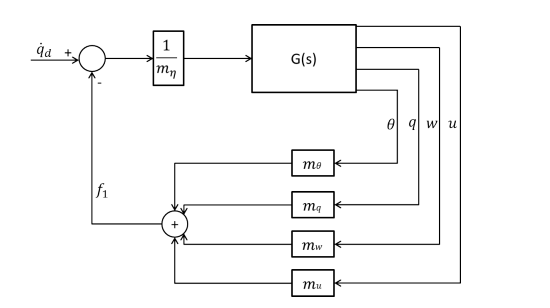
\includegraphics[width=15cm,height=10cm]{Оглавление/Part3/figures/САУ_ОД.png}
    \caption{Реализация динамической инверсии}
    \label{fig:САУ_ОД}
    \end{figure}
\subsection{Изучение робастности} 

Чтобы изучать робастность контроллера на основе обратной динамики мы проводили эксперементы с разными моделями продольного движения разных самолётов. 

\subsubsection{Модель (European SPS)} 
    $$\begin{bmatrix}
        -0.0110 & 0.0433 & 1.7295 & -7.1876\\ 
        -0.0691 & -0.6975 & -7.0678 & -54.8976\\ 
        0.00011 & 0.00116 & -0.35407 & 0.0911\\ 
        0 & 0 & 1 & 0
    \end{bmatrix} \cdot X=\begin{bmatrix}
        -0.4412\\ 
        -12.388\\ 
        -0.58446 \\ 
        0
\end{bmatrix} \cdot U=\dot{X}$$
\begin{center}
    Эксперименты с изменениями А и В
\end{center}

Суть этого эксперимента заключается в проверке характеристик надежности системы при изменении матрицы входных параметров $B$. Результаты эксперимента можно кратко изложить ниже.
    
\begin{figure}[H]
    \centering 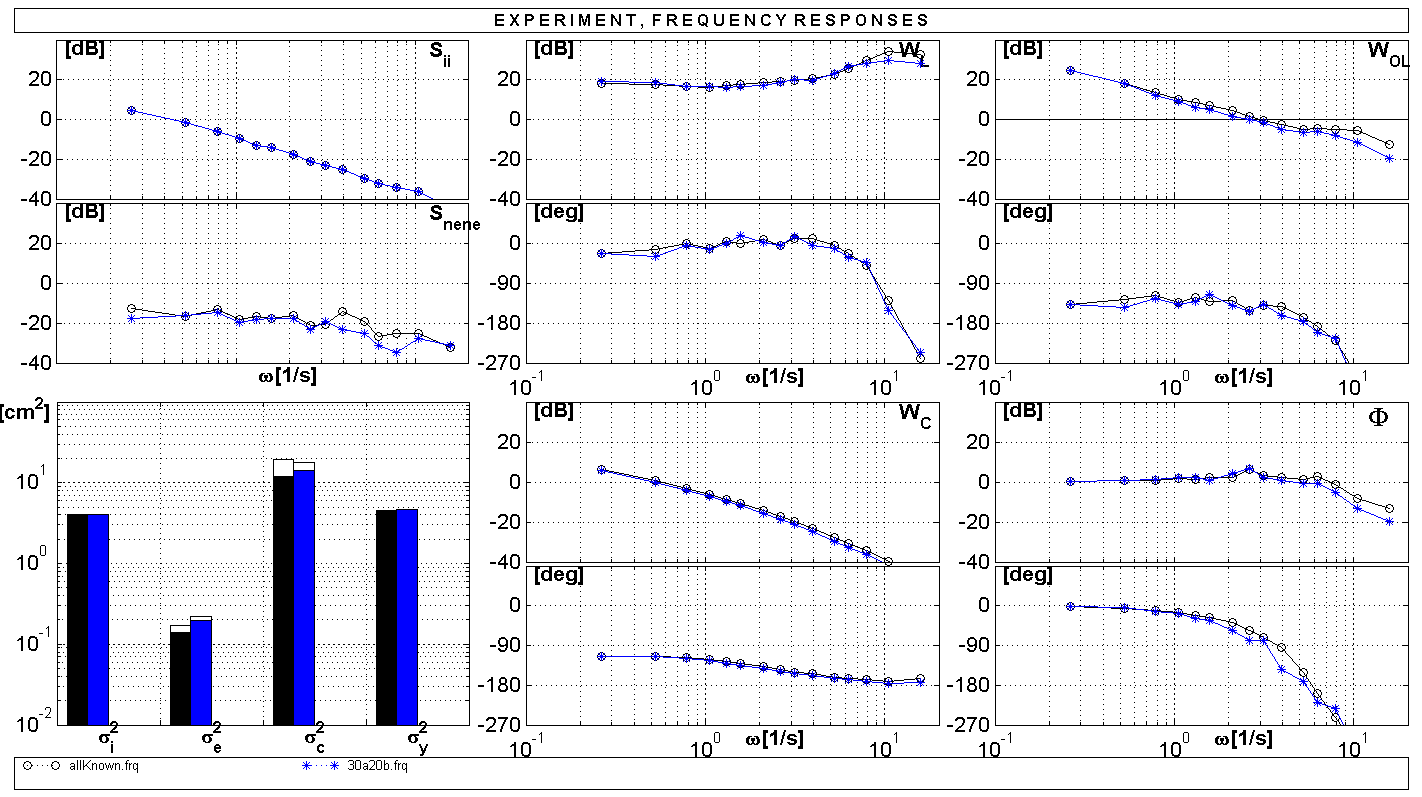
\includegraphics[width=17cm,height=15cm]{Оглавление/Part3/figures/chast2_20A30B.png}
    \caption{}
    \label{fig:Частотки второй Системы с изменением А и В}
    \end{figure}

    \begin{center}
        Эксперимент без PI 
    \end{center}



    Также мы подразумеваем, что мы имеем дело с $K_\text{ш} = -0,6$

    Из Рис. \ref{fig:Результаты экспериментов без PI}
    \begin{itemize}
        \item [-] c увеличением неточности знаний увеличивается $\sigma_e^2$
        \item [-] лётчик вводит меньшие усилия на ручку управления $\sigma^2_c$ 
        \item [-]  ...  
    \end{itemize}